\begin{exercise}{Photo aillée}{-1}{Spé}
{Optique géométrique}{lelay, centrale}

Une tête d'ail fait à peu près 7 cm de diamètre. La photographie reproduite ci-dessous a été prise à une distance $D$ de l'ail avec un appareil photographique assimilable à une lentille convergente de distance focale $f' = 50$~mm en utilisant un diaphragme de rayon $R$ et une pellicule de 24x36~mm placée à une distance $d$ de la lentille.

\begin{figure}[H]
    \centering
    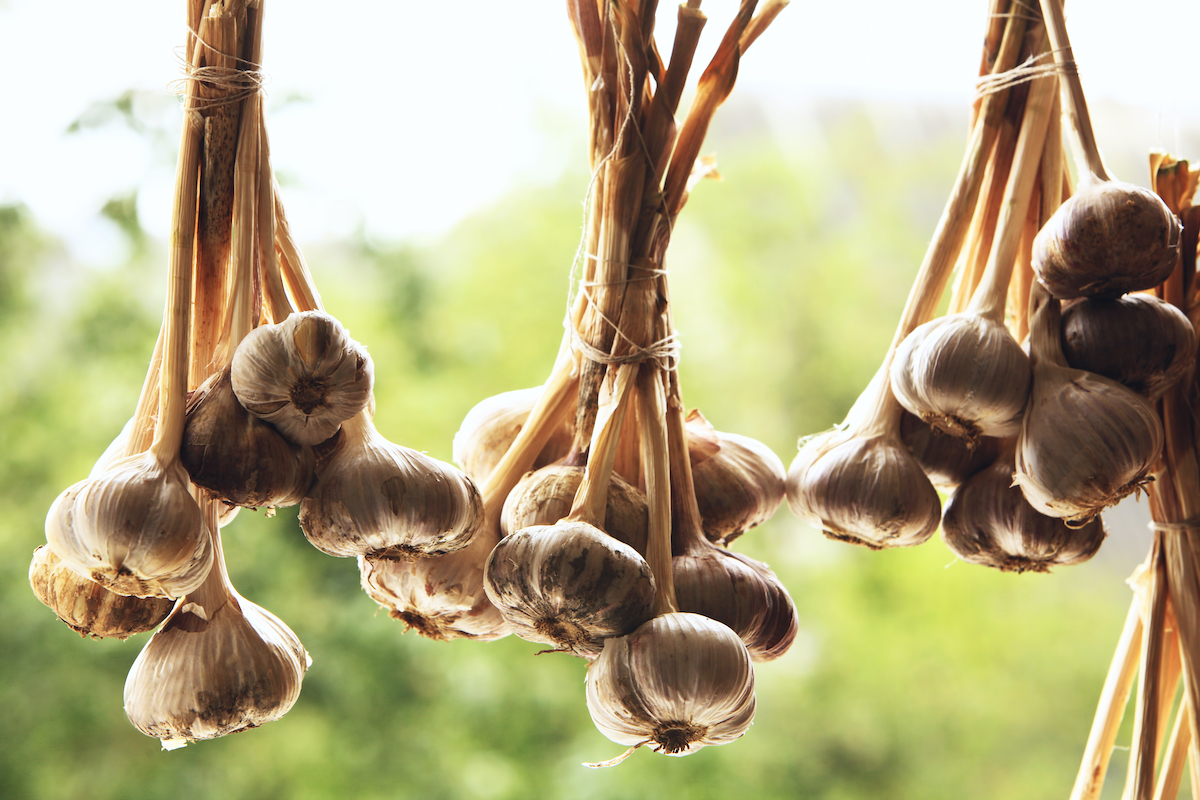
\includegraphics[width=.8\linewidth]{optique/optiquegeometrique/ail.jpg}
    \caption{Photographie d'une gousse d'ail.}
\end{figure}


\paragraph{Résolution de problème :}
\begin{questions}
    \question En vous aidant de la photographie fournie, déterminer la taille des gousses d’ail sur la pellicule. En déduire $d$ et $D$.
    \question On voit sur la photos des ronds clairs qui viennent d’objets au loin. Déterminer leur taille sur la pellicule, en déduire le rayon
du diaphragme $R$. Donner le nombre d'ouverture de l'appareil $\frac{f'}{2R}$.
    \question À quel phénomène aurait-on pu penser pour expliquer ronds ? Montrer quantitativement que ce n’est pas dû à cette cause.
    \question Quelle semble être la distance maximale jusqu’à laquelle on voit net ? En déduire la taille d’un élément photosensible sur cette
pellicule. Comparer à la résolution en pixels d’un appareil récent.
\end{questions}

\end{exercise}